\documentclass{article}

% if you need to pass options to natbib, use, e.g.:
    % \PassOptionsToPackage{numbers, compress}{natbib}
% before loading neurips_2020

% ready for submission
% \usepackage{neurips_2020}

% to compile a preprint version, e.g., for submission to arXiv, add add the
% [preprint] option:
    % \usepackage[preprint]{neurips_2020}

% to compile a camera-ready version, add the [final] option, e.g.:
\usepackage[final]{neurips_2020}

% to avoid loading the natbib package, add option nonatbib:
% \usepackage[nonatbib]{neurips_2020}

\usepackage[utf8]{inputenc} % allow utf-8 input
\usepackage[T1]{fontenc}    % use 8-bit T1 fonts
\usepackage{hyperref}       % hyperlinks
\usepackage{url}            % simple URL typesetting
\usepackage{booktabs}       % professional-quality tables
\usepackage{amsfonts}       % blackboard math symbols
\usepackage{nicefrac}       % compact symbols for 1/2, etc.
\usepackage{microtype}      % microtypography
\usepackage{graphicx}
\usepackage{subcaption}
\graphicspath{ {../plots} }

\title{Multi-Class Sentiment Analysis on Amazon Fine Food Reviews}

% The \author macro works with any number of authors. There are two commands
% used to separate the names and addresses of multiple authors: \And and \AND.
%
% Using \And between authors leaves it to LaTeX to determine where to break the
% lines. Using \AND forces a line break at that point. So, if LaTeX puts 3 of 4
% authors names on the first line, and the last on the second line, try using
% \AND instead of \And before the third author name.

\author{%
  Nikolaos Gounakis\\
  Department of Computer Science\\
  University of Crete\\
  Voutes University Campus, 700 13 Heraklion, Crete, Greece\\
  \texttt{nicolaig@csd.uoc.gr} \\
  % examples of more authors
  % \And
  % Coauthor \\
  % Affiliation \\
  % Address \\
  % \texttt{email} \\
  % \AND
  % Coauthor \\
  % Affiliation \\
  % Address \\
  % \texttt{email} \\
  % \And
  % Coauthor \\
  % Affiliation \\
  % Address \\
  % \texttt{email} \\
  % \And
  % Coauthor \\
  % Affiliation \\
  % Address \\
  % \texttt{email} \\
}

\begin{document}

\maketitle

\begin{abstract}
In Web applications it is useful to understand various concepts of text. 
One of them is the ability to understand if a piece of text provides a negative,
a positive or a neutral meaning. That can result to a new way of producing analytics 
for big companies when analyzing reviews or social media posts. In this study we compare
TF-IDF \cite{tfidf} and Doc2Vec \cite{doc2vec} for feature extraction of text data as 
the study \cite{studyPaper}. We evaluate them both on multi-class and binary classification
comparing 5 machine learning algorithms, using the Amazon Fine Food reviews 
dataset \cite{amzfood}.
\end{abstract}

\section{Introduction}
Text classification is challenging process. Machine learning techniques 
such as feature extraction enables us to map high dimensional data to a smaller 
number of variables. In our case text is the high dimensional input and using 
TF-IDF and Doc2Vec we will extract variables that represent this text in a 
lower dimension.

The Growth of modern web apps, such as Tweeter, Facebook and the million 
posts of users have brought in the surface the need of these big companies to 
analyze and gain information of these posts or reviews in our case. That will
enable the companies to have better analytics (analyze feedback) and also 
spotting users that create unwanted content in the platform. 

\section{Dataset: Amazon Fine Food Reviews}
\label{Dataset}
This dataset consists of reviews of fine foods from Amazon. 
The data span a period of more than 10 years, including all 568,454 reviews 
up to October 2012. Reviews include product and user information, ratings, and a plain text review. 
It also includes reviews from all other Amazon categories.
\url{https://www.kaggle.com/snap/amazon-fine-food-reviews}

The main columns of the dataset that we focus:
\begin{itemize}
  \item Score: ranges from 1 to 5 indicating good or bad review (int)
  \item Text: the actual review (String)
\end{itemize}

\section{Methodology}
As training data we will use the extracted features from the \textbf{Text} Column of the 
dataset \ref{Dataset} and labels from the \textbf{Score}.
We consider a \textbf{positive} review with a Score of 4 or 5, 
a \textbf{negative} review with a Score of 1 or 2 and a \textbf{neutral} review
with a Score of 3. We can see how the count distribution changes for the Score
from \ref{fig:Score5} to \ref{fig:Score3}. Now the lowest count belongs to the neutral 
reviews with a total of 42.640 reviews. We sample another 42.640 negative and 
positive reviews and constructing a dataset of size 127.920. 

\begin{figure}[h!]
  \centering
  \begin{subfigure}[b]{0.4\linewidth}
    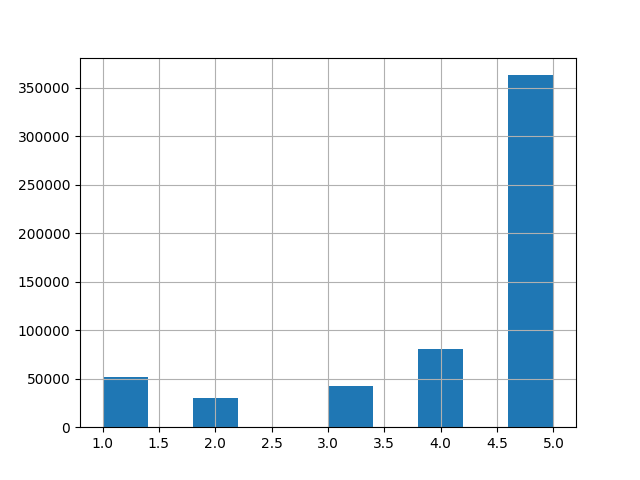
\includegraphics[width=\linewidth]{Score5.png}
    \caption{Score value distribution before}
    \label{fig:Score5}
  \end{subfigure}

  \begin{subfigure}[b]{0.4\linewidth}
    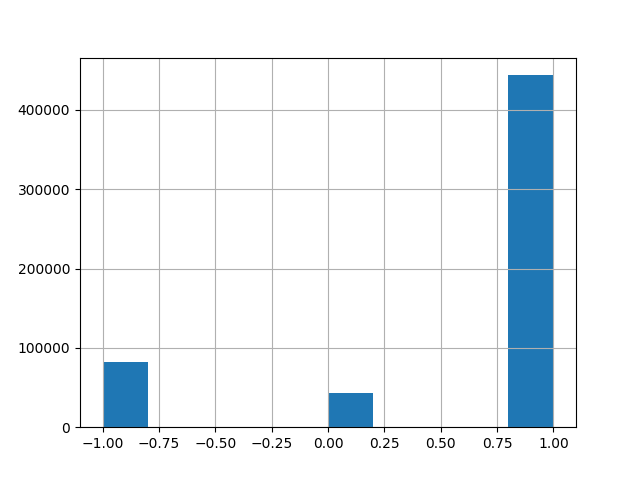
\includegraphics[width=\linewidth]{Score3.png}
    \caption{Score value distribution after dimensionality reduction}
    \label{fig:Score3}
  \end{subfigure}
  \caption{Score value count distribution}
\end{figure}

\subsection{Feature Extraction}
Now we are ready to perform the feature extraction using the two techniques 
we mention earlier (TF-IDF \cite{tfidf}, Doc2Vec \cite{doc2vec}). 
We must mention that due to the size of the features we couldn't make any plots
of the exported datasets.

\subsubsection{TF-IDF}
TF-IDF \cite{tfidf} is short form for term frequency-inverse document frequency.TF-IDF is
one of the largely used methods in information retrieval and text mining.TF-IDF is
a weight metric which determines the importance of word for that document.

We use the sklearn \cite{scikit-learn} implementation of the TF-IDF vectorizer.
We use the hyperparameters proposed by the authors of the paper \cite{studyPaper} with a slight
change to min\_df and max\_df,\. The configurtation is
displayed in table \ref{hyptfidf}.

We feed the vectorizer with the \textbf{Text} column, and extracting 638 features per row,
resulting in a 638*127.920 shape of the final dataset.

\begin{table}[h]
  \centering
  \begin{tabular}{ll}
  \hline
  min\_df       & 0.01                      \\
  max\_df       & 0.8 \\
  encoding      & utf-8                  \\
  sublinear\_df & True                   \\
  use\_idf      & True                   \\
  stop words    & English                \\ \hline
  \end{tabular}
  \caption{Hyper parameters for TF-IDF Vectorizer}
  \label{hyptfidf}
\end{table}

\subsubsection{Doc2Vec}

Is an extended version of word2vec, Doc2Vec model was put forward the study \cite{doc2vec} to improve 
the learning of embeddings from word to word sequences. Doc2Vec can be applied 
for word n-gram, sentence, paragraph or document. Doc2Vec is a set of 
approaches to represent documents as fixed length low dimensional vectors.

We used the Genism \cite{Genism} implementation of and the proposed hyperparameters \cite{studyPaper}
displayed in table \ref{hypdoc2vec}.

The output dataset consists of 100 features per row resulting in a 100*127.920 shape.

\begin{table}[h]
  \centering
  \begin{tabular}{ll}
  \hline
  min count   & 1    \\
  window size & 10   \\
  vector size & 100  \\
  sample      & 1e-4 \\
  negative    & 5    \\
  workers     & 7    \\
  dm          & 1    \\ \hline
  \end{tabular}
  \caption{Hyper parameters for Doc2Vec Vectorizer}
  \label{hypdoc2vec}
\end{table}

\section{Experiments}
In this section we evaluate the 5 classifiers (KNN, SVM-rbf, Naive Bayes, Random Forests, Logistic Regression) 
over the produced datasets. We used the sklearn implementations of the classifiers with default hyperparameters. 
Because of the large number of samples we randomly select 10.000 samples in total, 
with equal class distribution, and we perform a stratified 10-fold cross validation.
The metrics we compute are: Accuracy, f1 and AUC. 

\subsection{Multi-Class Classification}
\label{multiclass}
In multi-class classification the results were interesting. In table \ref{multiscore} we see that 
\textbf{SVM} and \textbf{Logistic Regression} outperform the rest classifiers with 
\textbf{SVM} having the highest scores. We see greater AUC than accuracies because it is 
calculated for each class and then the weighted average is computed considering the number of 
samples of each class.  

TF-IDF performs 45\% better than Doc2Vec in multi-class classification with the SVM classifier, but 
we see very low scores in general.
\begin{table}[h]
  \begin{tabular}{lllllll}
  \hline
  Feature Extraction Method & \multicolumn{3}{l}{TF-IDF}                          & \multicolumn{3}{l}{Doc2Vec}                         \\ \hline
                            & Accuracy        & F1              & AUC             & Accuracy        & F1              & AUC             \\ \hline
  KNN (n=5)                 & 47.990          & 46.228          & 65.965          & 39.580          & 39.367          & 56.897          \\
  SVM-rbf                   & \textbf{64.910} & \textbf{64.883} & \textbf{82.694} & \textbf{44.139} & \textbf{43.741} & \textbf{62.465} \\
  Logistic Regression       & 63.080          & 62.941          & 80.915          & 37.909          & 37.087          & 54.663          \\
  RF                        & 40.519          & 40.473          & 58.931          & 40.519          & 40.473          & 58.931          \\
  NB                        & 36.980          & 31.211          & 55.265          & 36.980          & 31.211          & 55.265          \\ \hline
  \end{tabular}
  \caption{Multi-Class Classification scores with weighted AUC}
  \label{multiscore}
\end{table}

\subsection{Binary Classification}
\label{binary}
Because of the low scores than the previous experiment performed we wanted to check how
the existence of the neutral class can affect the scores.

We removed the neutral class from the datasets keeping only
the negative and positive (Score values \{-1,1\}) and randomly selected 10.000 samples with
equal class distribution. We now perform a Binary classification. Again we used a stratified
10-fold cross validation and computed the same metrics. Because of the equal class distribution 
using stratified folds the AUC can be ignored.

In table \ref{binscore} we see again that the SVM classifier has the best overall performance.
In comparison with the Doc2Vec, TF-IDF is better by 31\%.

Binary Classification performance was better than multi-class by 29\%. That states, the 
neutral class was not well separable from the other classes and caused a problem.

\begin{table}[h]
  \begin{tabular}{lllllll}
  \hline
  Feature Extraction Method & \multicolumn{3}{l}{TF-IDF}                          & \multicolumn{3}{l}{Doc2Vec}                         \\ \hline
                            & Accuracy        & F1              & AUC             & Accuracy        & F1              & AUC             \\ \hline
  KNN (n=5)                 & 71.120          & 71.888          & 71.132          & 58.710          & 63.232          & 58.425          \\
  SVM-rbf                   & \textbf{83.670} & \textbf{83.569} & \textbf{83.668} & \textbf{63.540} & \textbf{66.232} & \textbf{63.374} \\
  Logistic Regression       & 82.780          & 82.684          & 82.778          & 57.980          & 63.065          & 57.657          \\
  RF                        & 81.580          & 81.435          & 81.577          & 59.949          & 60.927          & 59.924          \\
  NB                        & 79.260          & 79.566          & 79.267          & 54.190          & 63.736          & 53.533          \\ \hline
  \end{tabular}
  \caption{Binary Classification scores}
  \label{binscore}
\end{table}
  
\section{Colnclusions}

Considering the \ref{multiclass}, \ref{binary} an SVM with rbf kernel is preferable in this kind 
of situations, where features are extracted by a TF-IDF, Doc2Vec coming to an agreement
with the study \cite{studyPaper}. We can say that TF-IDF performs better in extracting 
features from review-like text. In \ref{binary} Binary classification we saw that the 
neutral class caused a problem in \ref{multiclass} multi-class classification. Thanks to that
in a future work we could focus in to making the neutral class more separable using a projection
or feature selection techniques. Finally, we could focus on tuning the SVM-rbf hyperparameters 
for even better accuracy.


\bibliographystyle{plain}
\bibliography{bib/report}


\end{document}